\chapter{Optimizaci\'on y paralelizaci\'on del filtro DNLM}
\label{ch:solucion}

En este cap\'itulo se presenta la paralelizaci\'on del filtro DNLM, con una comparaci\'on entre dos optimizaciones algor\'itmicas presentes en la literatura y sus respectivas versiones paralelas. La primera es una optimizaci\'on propuesta para el filtro DNLM, llamada DNLM-IIFFT. Se enfoca en disminuir la funci\'on de costo computacional mediante el uso de im\'agenes integrales y la transformada r\'apida de Fourier \cite{CalderonRamirez2017}. La segunda optimizaci\'on elegida es adaptada en este trabajo al filtro DNLM, debido a que fue presentada originalmente para el filtro NLM. Esta optimizaci\'on, en adelante DNLM-MOAS, acelera el c\'alculo de la funci\'on de pesado del filtro gracias al uso de un filtro de media m\'ovil, en adici\'on con el cambio en los ciclos de iteraci\'on y el aprovechamiento de la simetr\'ia de la funci\'on de pesado del filtro NLM \cite{Condat2010}. Ambas optimizaciones se detallan en la secci\'on \ref{ch:marco_opt}.

El paralelismo se emplea en dos formas: a nivel de tareas y a nivel de datos. En el caso del paralelismo a nivel de datos, este trabajo se enfoca en la vectorizaci\'on de la mayor cantidad de operaciones vectorizables presentes el algoritmo. Para esto se propone el uso de las primitivas de Intel para procesamiento de se\~nales e im\'agenes, llamadas \textit{Integrated Performance Primitives} (IPP). Las rutinas de esta biblioteca est\'an optimizadas para utilizar datos alineados en memoria y generar instrucciones SIMD vectorizadas. Estas instrucciones vectorizadas son aprovechadas por las unidades vectoriales presentes en la arquitectura Xeon Phi Knights Landing.



\section{Versiones del filtro DNLM a implementar}

Para lograr una correcta comparaci\'on entre las optimizaciones del filtro DNLM, se realiza la implementaci\'on de ambas optimizaciones DNLM-IIFT y DNLM-MOAS, sumadas a la versi\'on original del filtro DNLM que debe servir como punto base de comparaci\'on.

El funcionamiento del filtro DNLM se puede generalizar como un kernel $\psi_{\textrm{NLM}}$ que modifica a cada pixel de la imagen de entrada $U$, como se puede ver en (\ref{eq:weighted}) y \ref{eq:nlmfunc}. El kernel $\psi_{\textrm{NLM}}$ determina el valor del pixel filtrado, iterando sobre los pixeles de la ventana de b\'usqueda $\Omega$ con el fin de ponderar los vecindarios $\omega$. Una vez obtenido el peso del pixel, se multiplica por la imagen mejorada $U_{\textrm{USM}}$ producto del m\'etodo de \textit{Unsharp Mask} utilizado.  Finalmente, se normaliza el resultado para obtener la imagen final. 

El pseudoc\'odigo del filtro DNLM se muestra en la Figura \ref{fig:euclid}.

\begin{figure}[H]

\begin{algorithmic}[1]
\State $W\gets \Call{CreateMatrix}{U.size}$
\For{$i\gets 0, i < (U.rows - 1)$}
	\For{$j\gets 0, j < (U.cols - 1)$}
		\State $\Omega\gets \Call{GetCurrentPixelWindow}{i,j}$
        \State $E\gets \Call{CreateMatrix}{\Omega.size}$
        \State $\omega_{p}\gets \Call{GetPixelNeighborhood}{i,j}$
        \For{$n\gets 0, n < (\Omega.rows - 1)$}
        	\For{$m\gets 0, m < (\Omega.cols - 1)$}
        		\State $\omega_{m}\gets \Call{GetPixelNeighborhood}{n,m}$
                \State $E(n,m)\gets \Call{EuclideanDist}{\omega_m,\omega_p}$              
        	\EndFor 
        \EndFor 
        \State $W(i,j)\gets \Call{Average}{E}$
	\EndFor
\EndFor
\State \textbf{return} $W$
\end{algorithmic}
\caption{Pseudoc\'odigo del algoritmo del filtro DNLM}\label{fig:euclid}
\end{figure}


De la misma menera, se muestra el pseudoc\'odigo de las optimizaciones DNLM-IIFT y DNLM-MOAS en las Figuras \ref{fig:euclid2} y \ref{fig:euclid3}.

\begin{figure}[H]

\begin{algorithmic}[1]
\State $W\gets \Call{CreateMatrix}{U.size}$
\State $\SSI\gets \Call{IntegralImage}{U*U}$
\For{$i\gets 0, i < (U.rows - 1)$}
	\For{$j\gets 0, j < (U.cols - 1)$}
		\State $\Omega\gets \Call{GetCurrentPixelWindow}{i,j}$
        \State $\omega_{p}\gets \Call{GetPixelNeighborhood}{i,j}$
        \State $E\gets \Omega * \omega_{p}$ \Comment{Perform convolution}
        \For{$n\gets 0, n < (\Omega.rows - 1)$}
        	\For{$m\gets 0, m < (\Omega.cols - 1)$}
        		\State $E(n,m)\gets E(n,m) + SSI(i+n,j+m) + SSI(i,j)$              
        	\EndFor 
        \EndFor 
        \State $W(i,j)\gets \Call{Average}{E}$
	\EndFor
\EndFor
\State \textbf{return} $W$
\end{algorithmic}
\caption{Pseudoc\'odigo del algoritmo del filtro DNLM-IIFFT}\label{fig:euclid2}
\end{figure}

Se observa como disminuyen la cantidad de ciclos de iteraci\'on del algoritmo del filtro DNLM-IIFFT respecto a la versi\'on original, en su lugar se realiza una convoluci\'on entre la ventana de b\'usqueda $\Omega$ y el vecindario $\omega_{p}$, reduciendo la funci\'on de costo del algoritmo. 


\begin{figure}[H]

\begin{algorithmic}[1]
\State $W\gets \Call{CreateMatrix}{U.size}$
\For{$dn\gets 0, dn < (\Omega.len/2 - 1)$}
	\For{$dm\gets 0, dm < (\Omega.len/2 - 1)$}
		\If	{$dn == 0 \And dm == 0$}
			\State $W\gets W + \Call{Ones}{W.size}$
		\Else
			\State $SSD\gets \Call{CalcSSD}{U,dn,dm}$ 
			\State $E\gets SSD * \Call{Ones}{W.size}$ \Comment{Perform convolution}
			\State $W\gets W + \Call{Exp}{E/h}$ 
		\EndIf
	\EndFor
\EndFor
\State \textbf{return} $W$
\end{algorithmic}
\caption{Pseudoc\'odigo del algoritmo del filtro DNLM-MOAS}\label{fig:euclid3}
\end{figure}


En el filtro DNLM-MOAS la reducci\'on es a\'un m\'as dr\'astica: Se itera sobre  las distancias dentro de la ventana de b\'usqueda, en lugar de iterarar sobre los pixeles de la imagen. 



\section{Vectorizaci\'on}

El uso de la biblioteca IPP es necesario para lograr la vectorizaci\'on de las operaciones del filtro sin tener que recurrir al uso de instr\'insicas. Esto premite obtener un c\'odigo m\'as legible y f\'acil de mantener. 

La biblioteca IPP implementa un despachador que selecciona atom\'aticamente el conjunto de instruccions SIMD espec\'ifico para las rutinas de la biblioteca, de acuerdo a las caracter\'isticas del procesador \cite{IntelCorporation2017}.  Sin embargo, tambi\'en permite establecer un conjuntos de instrucciones SIMD espec\'ifico \cite{IntelCorporation2017}. Esto resulta \'util para comprobar la diferencia en rendimiento entre diferentes conjuntos de instrucciones SIMD seg\'un se requiera.


\section{Paralelizaci\'on}

El filtro DNLM tiene la ventaja de poder realizar el filtrado de cada pixel de manera independiente. Esto se puede intuir de la funci\'on de filtrado (\ref{eq:weighted}). El resultado es un alto nivel de paralelismo, con un grado de granularidad propicio para distribuir la carga de procesamiento en los n\'ucleos del procesador, como se observa en la Figura \ref{fig:parallel_figure}. 



\begin{figure}[H]
   \centering
   \caption[Diagrama de distribuci\'on de tareas paralelas]{Diagrama de distribuci\'on de tareas para la paralelizaci\'on del filtro DNLM}
   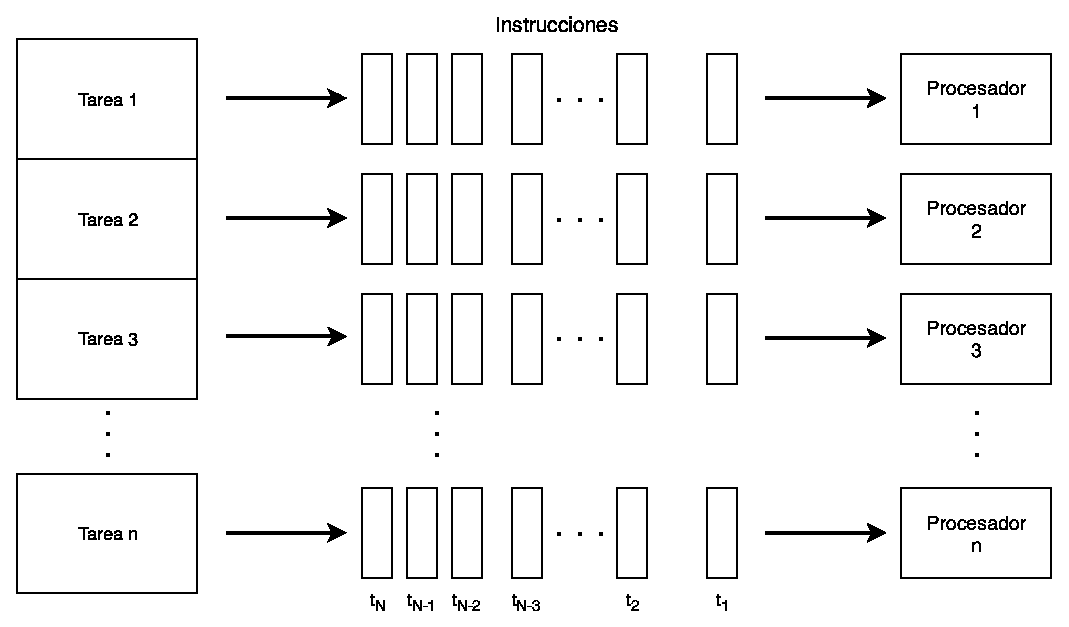
\includegraphics[width=0.8\textwidth]{parallel_figure}
   \label{fig:parallel_figure}
 \end{figure}
 

Existen m\'ultiples enfoques de paralelizaci\'on propuestos en la literatura que han demostrado una alta aceleraci\'on del algoritmo de filtrado, como lo muestra la Tabla \ref{method_table}. 


\begin{table}
\caption{M\'etodos previos de implementaciones paralelas para el filtro NLM. Se muestra \'unicamente la aceleraci\'on m\'axima respecto a la versi\'on secuencial no optimizada del filtro.}
\begin{tabularx}{1\linewidth}{X X X X} 
\hline
Implementaci\'on & Arquitectura & M\'etodo & Aceleraci\'on \\ [0.5ex]
 \hline\hline
 Coupe et al. \cite{coupe2006fast} &  8 Intel Xeon CPU & Biblioteca de Hilos & 50x\\
 Darbon et al. \cite{Darbon2008} &  8 Dual-Core AMD Opteron CPU & Instrucciones Vectorizadas & 110x\\
 Mingliang et al. \cite{mingliang2016medical} &  NVIDIA Quadro FX 480 & CUDA & 40x\\
Gossens et al. \cite{goossens2010gpu} &  NVIDIA GeForce 9600 GT & DirectX & 402x\\
Marques and Pardo. \cite{marques2013implementation} &  NVIDIA GeForce GTX 680 & CUDA & 718x\\ 
Shi et al. \cite{shi2015optimized} &   1024 n\'ucleos SuperMUC & MPI & 740x\\
Nguyen et al. \cite{nguyen2016medical} &   8 Intel Xeon CPU & MPI y PThreads & 148x\\
Nguyen et al. \cite{nguyen2016medical} &   8 NVIDIA Tesla C2050 & MPI y CUDA & 510x\\
Zhu et al. \cite{zhu2016parallel} &  Intel Xeon Phi 7110P & OpenMP & 87x\\
Zhu et al. \cite{zhu2016parallel} &  Intel Xeon Phi 7110P & OpenCL & 108x\\
Huang et al. \cite{huang2017parallel} &  Intel Xeon Phi & OpenMP & 32x\\
\end{tabularx}
\label{method_table}
\end{table}

La primera implementaci\'on paralela encontrada en la literatura se realiz\' mediante m\'ultiplles hilos de ejecuci\'on para procesar im\'agenes m\'edicas en 3D, con la ayuda de un servidor y 8 procesadores Xeon \ \cite{coupe2006fast}. Seguidamente, se utiliza una arquitectura SIMD para paralelizar el filtro en un servidor con 8 procesadores AMD Opteron de doble n\'ucleo \cite{Darbon2008}. Adem\'as, implementaciones en GPU han empleado la optimizaci\'on propuesta por Gossens en DirectX \cite{marques2013implementation} y la optimizaci\'on propuesta por Condat en CUDA \cite{mingliang2016medical,goossens2010gpu}, las cuales muestran mayores aceleraciones que las implementaciones en CPU. Otra implementaci\'on con una aceleraci\'on ligeramente mayor a la obtenida por Marques y Pardo \cite{marques2013implementation} es conseguida en un sistema distribuido con 1024 n\'ucleos de procesamiento \cite{shi2015optimized}. Una implementaci\'on m\'as compleja combina MPI con P-Threads y MPI con CUDA para alcanzar una aceleraci\'on a\'un mayor \cite{nguyen2016medical}. Finalmente, dos implementaciones del filtro para plataformas Xeon Phi \cite{zhu2016parallel,huang2017parallel} y OpenCL \cite{zhu2016parallel}.

Si bien la aceleraci\'on obtenida con GPU es usualmente mayor a las reportadas con la plataforma Xeon Phi, \'esta \'ultima tiene la ventaja de proveer un estilo de programaci\'on sencillo y flexible, ya que utiliza el set de instrucciones X86 \cite{huang2017parallel}. 